\documentclass[12pt,]{article}
\usepackage[utf8]{inputenc}
\usepackage[T1]{fontenc}
\usepackage{mathptmx}
\usepackage{geometry}
\usepackage{mathtools}
\usepackage[english]{babel}
\usepackage{graphicx}
\usepackage[os=win]{menukeys}
\usepackage[figurename=Gambar]{caption}
\usepackage{hyperref}
\usepackage{minted}
\usepackage{xcolor}
\usepackage{tikz}
\usepackage[yyyymmdd,hhmmss]{datetime}

\newcommand{\ShowOsVersion}{
	\immediate\write18{\unexpanded{foo=`uname -sro` && echo "\\\verb${foo}" > tmp.tex}}
	\input{tmp}\immediate\write18{rm tmp.tex}
}

\newcommand{\ShowTexVersion}{
	\immediate\write18{\unexpanded{foo=`pdflatex -version | head -n1` && echo "\\\verb${foo}" > tmp.tex}}
	\input{tmp}\immediate\write18{rm tmp.tex}
}

\addto\captionsenglish{\renewcommand{\contentsname}{Daftar Isi}}

\hypersetup{
	colorlinks=true, %set true if you want colored links
	linktoc=all,     %set to all if you want both sections and subsections linked
	linkcolor=blue,  %choose some color if you want links to stand out
}

\geometry{
	a4paper,
	left=15mm,
	right=10mm,
	top=10mm,
	bottom=10mm,
}

\title{\Large \bf
	Dokumen Teknis dan Laporan Sementara Development Instrumen PikoAkustik
}

\author{Achmadi ST MT}

\date{}

\definecolor{LightGray}{gray}{0.9}

\begin{document}

	\maketitle
	\thispagestyle{empty}
	\pagestyle{empty}
	
	\begin{figure}[!ht]
		\centering
		
\includegraphics[width=250pt]{images/yerba.png}
	\end{figure}
	
	\vspace*{125px}
	\noindent This report written using: \\
	OS : \ShowOsVersion \\
	TeX : \ShowTexVersion \\
	Update: {\today} at \currenttime \\
	
	\noindent Document Tex Source:\\
	\url{https://github.com/mekatronik-achmadi/my_latexbook/tree/master/Laporan/pikoakustik}
	
	\newpage
	\mbox{}
	
	\newpage
	(catatan: Daftar Isi dan Index bisa diklik)
	\tableofcontents
	
	\newpage
	\mbox{}
	
	\newpage
	\section{Project Repository}
	
	Seluruh design dan codebase untuk development di-\textit{dump} di repository yg beralamat:\\
	\url{https://github.com/VibrasticLab/pikoakustik}:\\
	
	Untuk saat ini pada fase versi development, repository bebas di-\textit{fork} atau diambil,
	dengan syarat:
	\begin{itemize}
		\item Penggunaan komersial masih dibatasi dan wajib notifikasi ke pemilik repository,
		yaitu Laboratorium Vibrasi dan Akustik Departemen Teknik Fisika ITS.
		
		\item Sesuai aturan lisensi GPLv2, maka diwajibkan mengembalikan modifikasi/perbaikan 
		yang dilakukan pada versi \textit{fork} baik dengan \textit{pull-request} atau email \textit{patch}.
	\end{itemize}
	
	\newpage
	\mbox{}
	
	\newpage
	\section{Versi Development/Testing}
	
	Berikut adalah penjelasan detil dan dokumentasi teknis untuk versi development:
	
	\subsection{Desain Platform}
	
	Berikut adalah detil desain platform untuk setiap modul/komponen.
	
	\subsubsection{Diagram Overview}
	
	Berikut diagram overview platform:
	
	\begin{figure}[!ht]
		\centering
		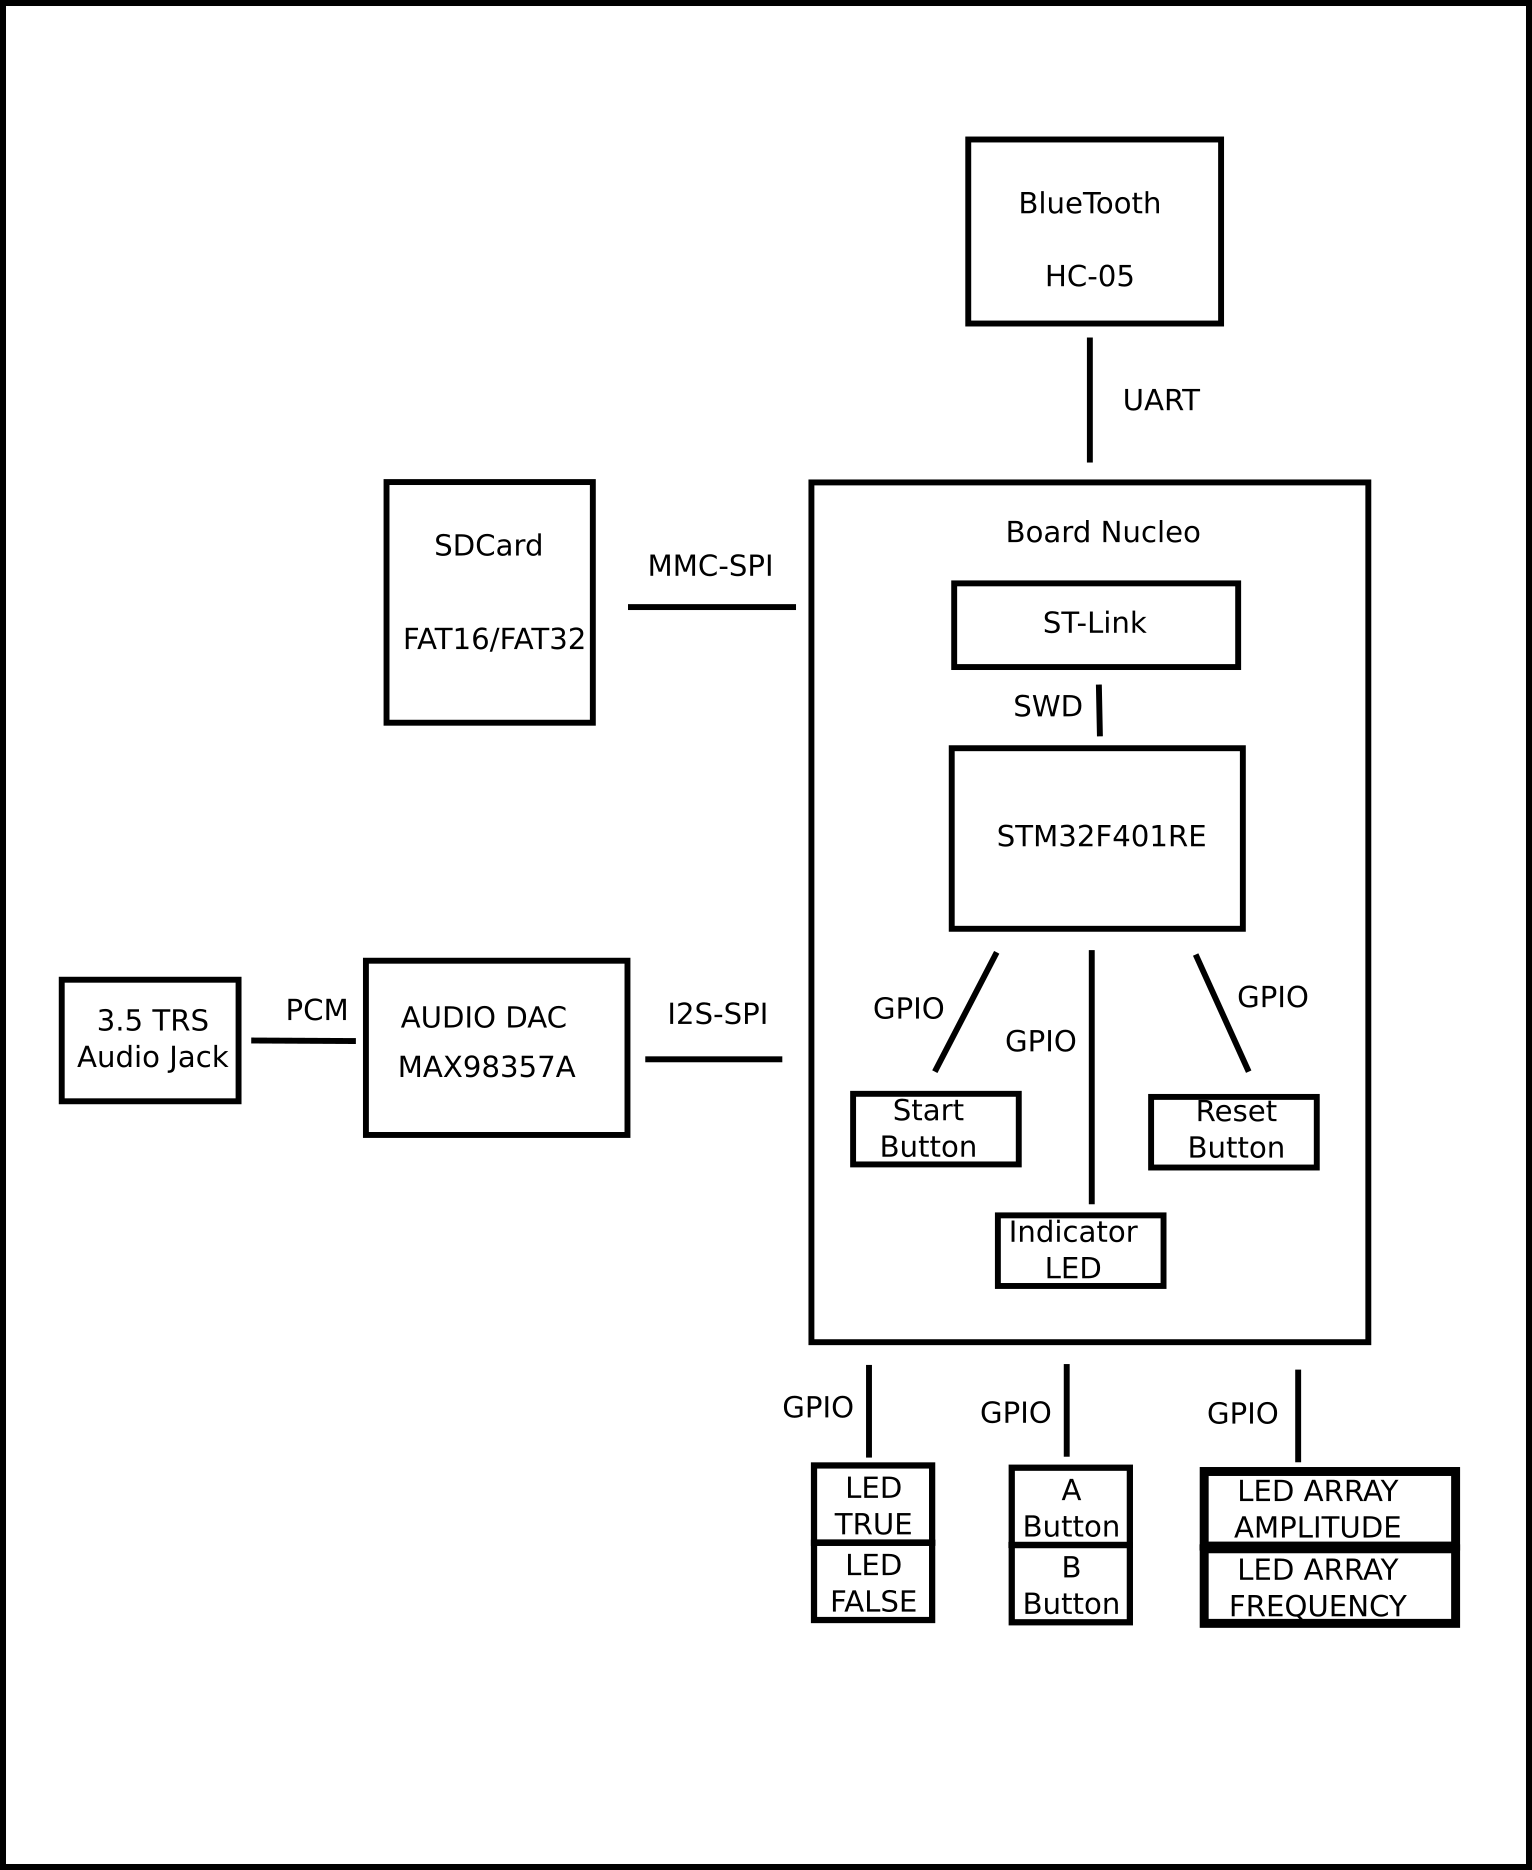
\includegraphics[width=400pt]{images/overview}
	\end{figure}
	
	\newpage
	\subsubsection{Board Nucleo STM32F401RE}
	
	Board Nucleo STM32F401RE adalah \textit{development-board} yang diproduksi oleh ST Microelectronic
	dan dipasarkan di Indonesia dengan harga terjangkau.
	Pertimbangan memilih board ini antara lain:
	\begin{itemize}
		\item Keseluruhan board hanya membutuhkan standar tegangan VDD (3,3v) dan VCC (5v) dengan draw arus rendah.
		Sehingga cocok untuk development instrumen tipe battery-operated.
		
		\item Board Nucleo menyediakan layout pin Arduino dan juga sekaligus ST-Morpho.
		Sehingga fleksibel untuk tahap development.
	
		\item Tersedia embedded ST-Link untuk download binary dan debugging.
	\end{itemize}

	Sedangkan pertimbangan memilih CPU STM32F401RE antara lain:
	\begin{itemize}
		\item Arus quiescent hanya 2,4uA sehingga hemat energi/battery.
		\item CPU Frequency 84MHz sehingga mampu multithreading.
		\item Tersedia protokol standar Audio I2S melalui protokol SPI.
		\item Tersedia internal DSP.
		\item Tersedia standar UART yang dapat dikontrol DMA.
		\item Tersedia integrasi DMA dan MMC-SPI untuk kebutuhan I/O SDCard.
		\item Frekuensi GPIO hingga 100MHz.
	\end{itemize}

	\begin{figure}[!ht]
		\centering
		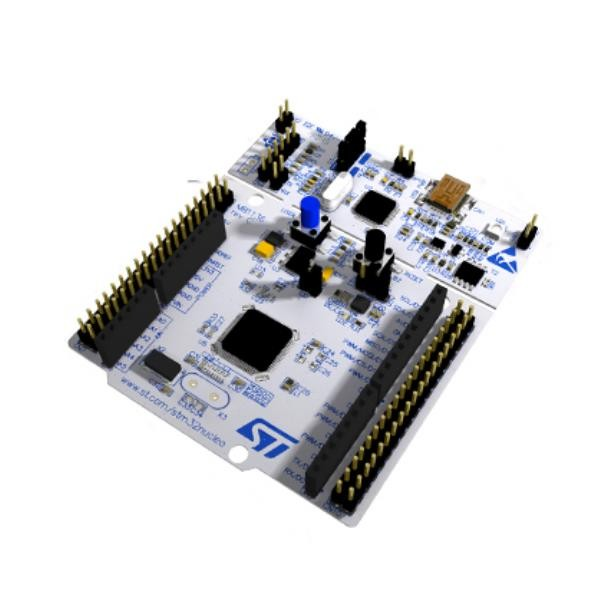
\includegraphics[width=300pt]{images/nucleo-f401re}
	\end{figure}

	Module ini dapat dibeli di Digiware-Store dengan harga Rp.202.000,-.\\
	\url{https://digiwarestore.com/en/microcontroller-dev-tools/nucleo-f401re-442175.html}
	
	\newpage
	\subsection{MAX98357A}
	
	Modul chip MAX98357A adalah modul Audio DAC yang dikomunikasi dengan chip STM32F401RE melalui protokol Audio I2S.
	Pertimbangan memilih chip ini untuk Audio DAC antara lain:
	\begin{itemize}
		\item Jangkauan resolusi 16bit.
		\item Tidak membutuhkan input sinyal MCLK.
		\item Jangkauan Sampling Rate 8kHz hingga 96kHz.
		\item Filterless Class D output.
		\item Tersedia pilihan Gain dari 3dB hingga 15dB.
		\item Menerima sinyal I2S tipe Left-Right maupun Mono.
	\end{itemize}

	Module ini dapat dibeli di Digiware-Store dengan harga Rp.141.000,-.\\
	\url{https://digiwarestore.com/en/mic-speaker-buzzer/amplifier-ic-development-tools-i2s-3w-class-d-amp-breakout-max98357a-3006-441053.html}
	
	\begin{figure}[!ht]
		\centering
		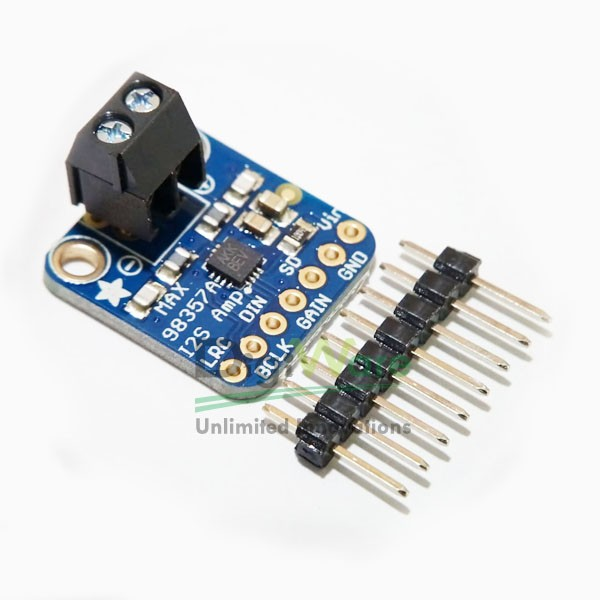
\includegraphics[width=300pt]{images/max98357}
	\end{figure}
	
	\newpage
	\subsection{SDCard}
	
	Untuk kebutuhan storage data atau streaming file media, digunakan module SDCard melalui protokol MMC-SPI dan emulasi filesystem dengan FatFS.
	Kombinasi MMC-SPI dan FatFS mampu meng-\textit{handle} baik MMC hingga SDHC asalkan tersedia protokol SPI dengan SCK 400kHz.
	
	Untuk SDCard holder ukuran MicroSD dapat dibeli di di Digiware-Store dengan harga Rp.41.000,-.\\
	\url{https://digiwarestore.com/en/connector/micro-sd-connector-push-push-8p-smt-r-a-dm3bt-dsf-pejs-919160.html}\\
	
	\begin{figure}[!ht]
		\centering
		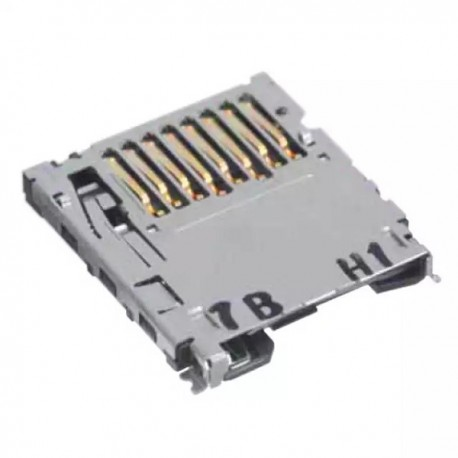
\includegraphics[width=200pt]{images/microsd}
	\end{figure}
	
	Sedangkan untuk SDCard sendiri dapat dibeli dimanapun semisal merek VGen di Sakinah Mart seharga Rp.65.000,-
	\begin{figure}[!ht]
		\centering
		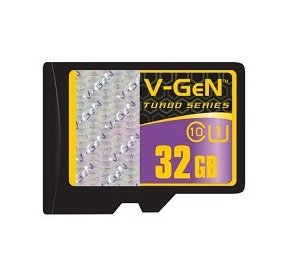
\includegraphics[width=200pt]{images/vgensdcard}
	\end{figure}

	\newpage
	\subsection{Bluetooth HC-05}
	
	Modul Bluetooth HC-05 adalah modul yang menyediakan \textit{interface} serial melalui emulasi di protokol BlueTooth.
	Melalui modul ini, instrumen dapat berkomunikasi dalam standar baudrate 9600 dengan perangkat mobile lain seperti Smartphone maupun Laptop.
	
	\begin{figure}[!ht]
		\centering
		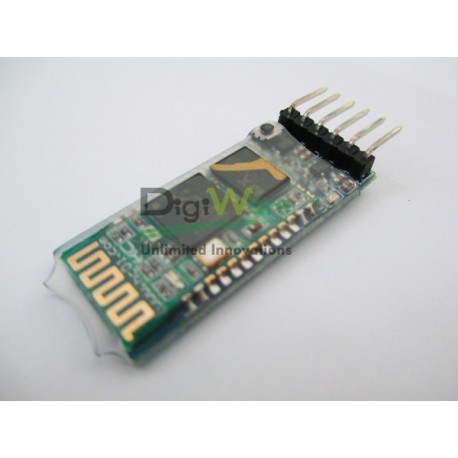
\includegraphics[width=200pt]{images/hc05}
	\end{figure}
	
	Modul ini dapat dibeli di di Digiware-Store dengan harga Rp.68.000,-.\\
	\url{https://digiwarestore.com/en/bluetooth/hc-05-bluetooth-module-432241.html}
	
	\subsection{Komponen Pendukung}
	
	Berikut adalah beberapa komponen pendukung yang tidak memiliki spesifik kebutuhan.
	
	\subsubsection{Jack Audio}
	
	Jack Audio yang dipilih adalah tipe 3.5mm TRS.
	Dapat dibeli di Digiware Store seharga Rp.4000.
	
	\begin{figure}[!ht]
		\centering
		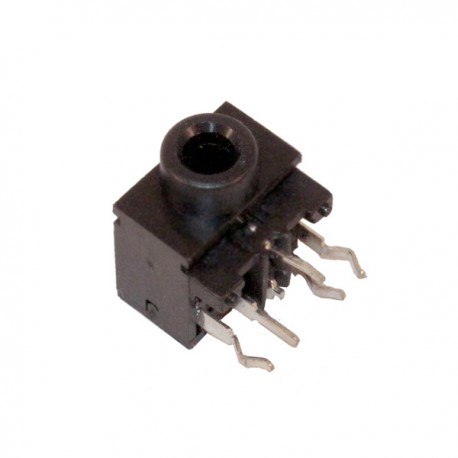
\includegraphics[width=150pt]{images/jackaudio}
	\end{figure}

	\newpage
	\subsubsection{LED}
	
	Led indikator yang digunakan adalah tipe SMT 0805.
	Dapat dibeli di Akhi Shop seharga Rp.200 per biji.
	Dibutuhkan total 14 LED sehingga total harga Rp.2800.
	
	\begin{figure}[!ht]
		\centering
		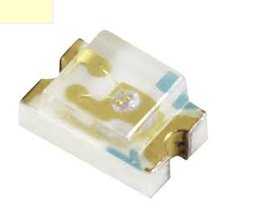
\includegraphics[width=150pt]{images/led0805}
	\end{figure}

	\subsubsection{PushButton}
	
	Led indikator yang digunakan adalah tipe SPDT 4P.
	Dapat dibeli di toko komponen elektronik terdekat dengan harga kisaran Rp.2000,00
	
	\begin{figure}[!ht]
		\centering
		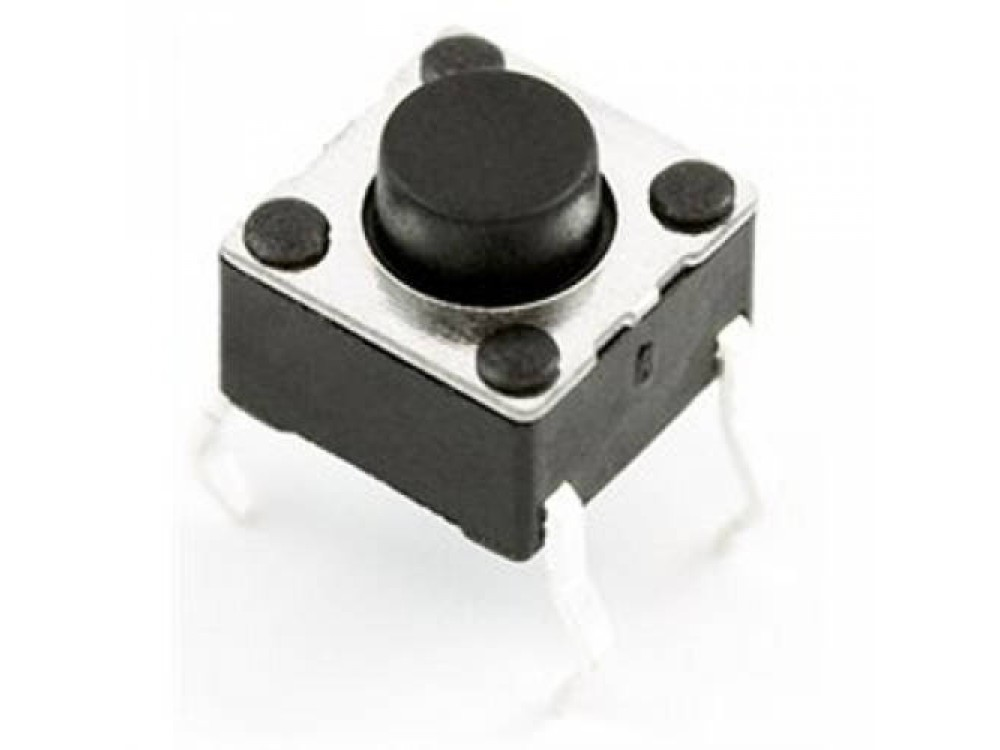
\includegraphics[width=150pt]{images/button}
	\end{figure}

	\newpage
	\subsection{MainBoard}
	
	MainBoard adalah modul/shield untuk menjadi wadah komunikasi board Nucleo dengan semua modul lain.
	Desain KiCAD dapat di download di:\\
	\url{https://github.com/VibrasticLab/pikoakustik/tree/master/stm32f401nucl/piko_stm32f4nucl}
	
	\begin{figure}[!ht]
		\centering
		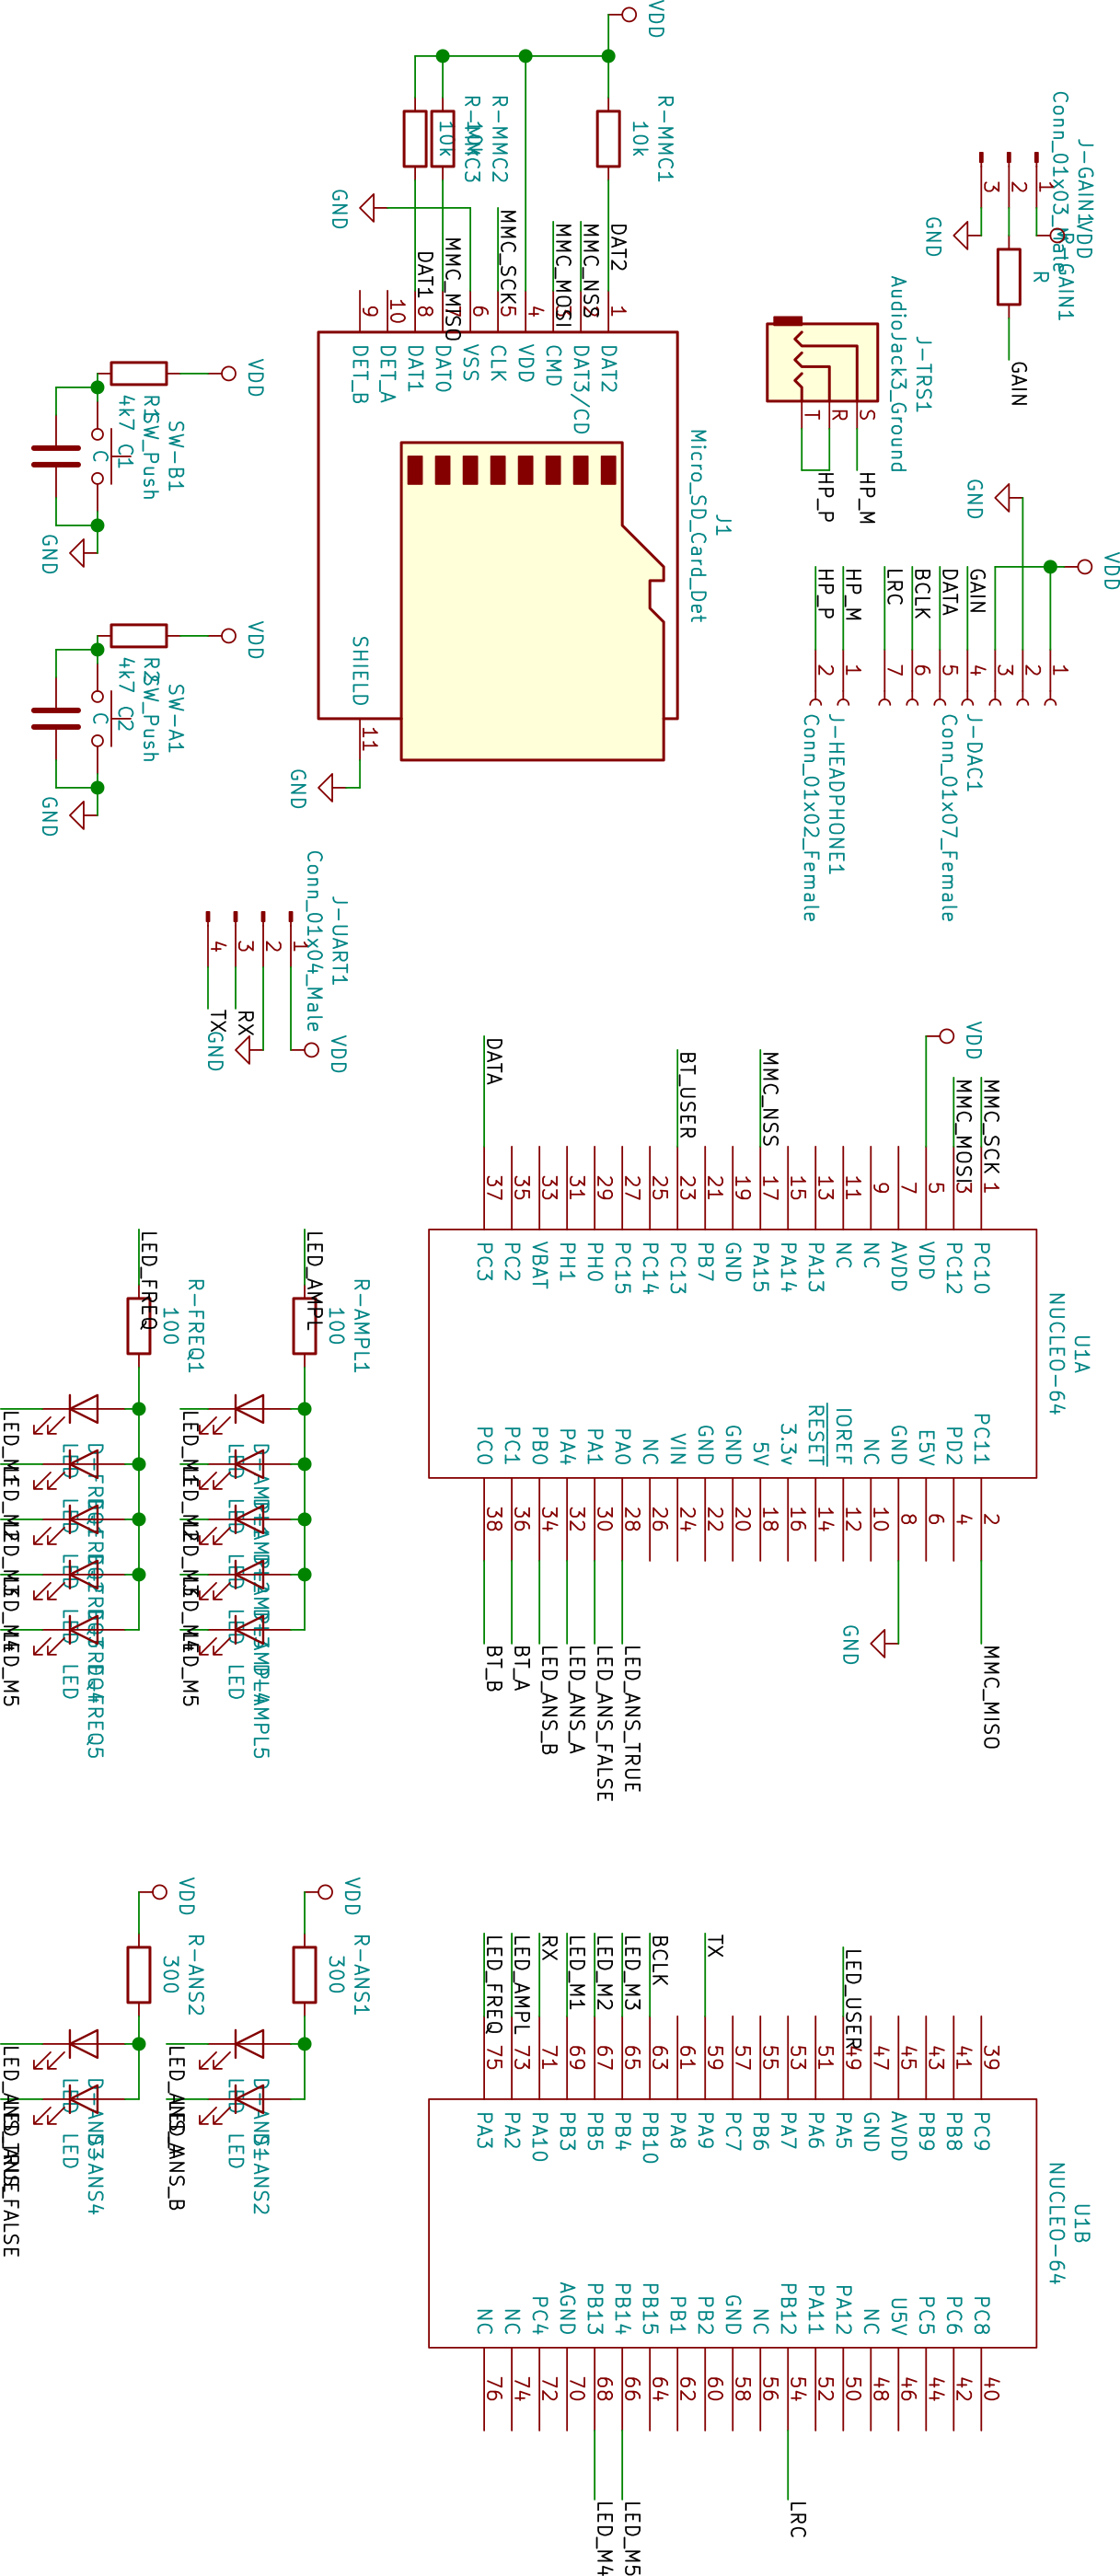
\includegraphics[width=300pt]{images/board}
	\end{figure}

	\newpage
	Layout Top:
	\begin{figure}[!ht]
		\centering
		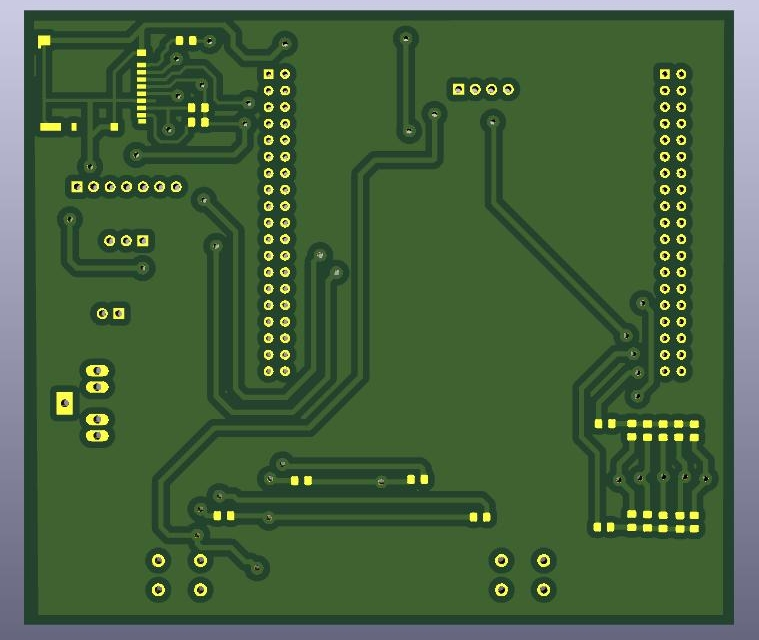
\includegraphics[width=400pt]{images/top}
	\end{figure}

	Layout Bottom:
	\begin{figure}[!ht]
		\centering
		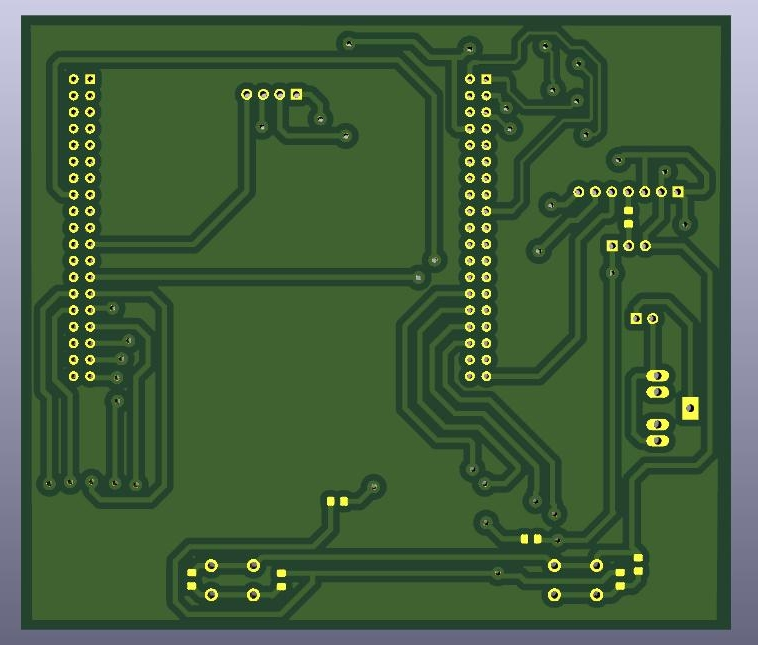
\includegraphics[width=400pt]{images/bottom}
	\end{figure}

	\newpage
	\subsection{Actual Development}
	
	Beikut adalah beberapa dokumentasi aktual hasil development:
	
	\newpage
	\mbox{}
	
	\newpage
	\subsection{Firmware}
	
	Untuk fase development, seluruh firmware yang tersedia masih tahap implementasi peripheral tanpa aplikasi.
	URL untuk source: \url{https://github.com/VibrasticLab/pikoakustik/tree/master/stm32f401nucl/}
	
	\subsubsection{Library}
	
	Beberapa Project lain yang menyediakan pustaka untuk development firmware:
	\begin{itemize}
		\item ChibiOS/RT buatan Giovanni D. Sirrio. Menyediakan pustaka untuk driver HAL dan kernel multithreading.
		\item FatFS buatan Chem Echan. Menyediakan pustaka pustaka untuk emulasi filesystem FAT16/FAT32.
	\end{itemize}

	\subsubsection{Wave Generation}
	 
	 Berikut adalah bagian firmware Sine Wave Generation yang secara diskrit dalam bahasa C.
	 Mengingat protokol I2S menulis data bit DAC dalam rentang buffer tertentu, maka langkah yang perlu diterapkan:
	 \begin{enumerate}
	 	\item Buat Array untuk 1 siklus (2$\pi$) diskrit sinusoidal dengan rentang amplitud 16bit dan sampling rate 44100
	 	\item Atur panjang array buffer sebanyak multiplikasi panjang array untuk 1 siklus.
	 	\item Feed buffer ke DMA yang mengontrol I2S
	 \end{enumerate}
	 
	 Fungsi untuk mendapatkan 1 siklus array
	 \begin{minted}[frame=lines,framesep=2mm,fontsize=\footnotesize,bgcolor=LightGray]{c}
uint16_t onewavelen(double FR,int AMP){
	double x,y;
	
	uint8_t neg_a = 0,neg_b = 0;
	uint8_t phase = 0;
	uint8_t stop = 0;
	uint16_t sample;
	
	uint16_t i = 1;
	
		while(stop==0){
		x = (double) i / (double) SAMPLING_RATE;
		y = sin(2.0 * 3.14159 * FR * x) + 1;
		sample = (uint16_t) AMP * 0.2 * y;
		
		i++;
		
		if(sample == 2000){ phase++;}
		else if(sample > 2000){ neg_b = 0;	}
		else if(sample < 2000){ neg_b = 1;	}
		
		if(neg_b != neg_a){
			phase=phase+1;
			if(phase==2){ ;stop=1;	}
			neg_a = neg_b;
		}
		else if(neg_b == neg_a){ neg_a = neg_b; }
		
		if(i==NUM_SAMPLES){	stop=1;	}
	};
	
	return i;
}
	 \end{minted}
	 
	 Dan fungsi untuk membuat sample yang akan digunakan (sesuai buffer untuk I2S):
	 \begin{minted}[frame=lines,framesep=2mm,fontsize=\footnotesize,bgcolor=LightGray]{c}
void sample_prep(
double FR, // Frequency (Hz)
double DUR, //Duration (s)
int AMP) //Amplitudo
{
 	double x,y;
 	
 	uint16_t waveone,wavenum,wavelen;
 	uint16_t sample;
 	
 	waveone = onewavelen(FR,AMP);
 	wavenum = (uint16_t) NUM_SAMPLES/waveone;
 	wavelen = NUM_CHANNELS * wavenum * waveone;
 	
 	uint16_t i = 1;
 	sine_sample[0] = AMP * 0.2;
 	
 	play_duration = DUR;
 	
 	for(i=1;i<I2S_BUF_SIZE;i++){
 		x = (double) i / (double) SAMPLING_RATE;
 		y = sin(2.0 * 3.14159 * FR * x) + 1;
 		sample = (uint16_t) AMP * 0.2 * y;
 		
 		sine_sample[i] = sample;
 		if(NUM_CHANNELS==2){ sine_sample[i+1] = sample; }
 	};
 	
 	i2scfg.size = wavelen;
}
	 \end{minted}
	 
	Dan fungsi untuk feed ke I2S sehingga wave akan di-\textit{play} sepanjang durasi:
	\begin{minted}[frame=lines,framesep=2mm,fontsize=\footnotesize,bgcolor=LightGray]{c}
void wave_test(void){
	i2sStart(&I2SD2, &i2scfg);
	i2sStartExchange(&I2SD2);
	
	chThdSleepMilliseconds(play_duration * 200);
	
	i2sStopExchange(&I2SD2);
	i2sStop(&I2SD2);
}
	\end{minted}
	
	\subsubsection{Peripheral: I2S}
	\subsubsection{Peripheral: MMC}
	\subsubsection{Peripheral: UART-Shell}
	\subsubsection{Peripheral: LED Indicator}
	\subsubsection{Peripheral: User Button}
	\subsubsection{Top-Down Program Firmware}
	\subsubsection{Main-Flow Program Firmware}
	
	\newpage
	\section{Versi End User}

\end{document}
